\subsection{Spark [VI]}

Spark is a framework for distributed data processing \cite{Zaharia2010} \cite{Zaharia2013} \cite{Spark1} \cite{Spark2}.
It provides a tool to work with large datasets and streams of data, and to make complex queries on this data.
Spark has several abstractions for representation of data and streams.
The first one - Resilient Distributed Dataset (RDD) - is an object, distributed in the cluster, that contains data to process.
Another one is a Shared Variable - variable, that can be used among the cluster as a counter or lookup table.
One more abstraction is a Discretized Stream (DStream) - representation of a data stream also in a distributed fashion.

\subsubsection{Data model and batch processing}

To initialize Spark you first create a SparkContext object, that is responsible for a connection of your program to Spark.
It allows to specify properties of your application, and also options of how Spark should run, for example in local mode or on the cluster.
SparkContext gives an access to different parameters and properties of execution environment.

\textit{Resilient Distributed Datasets}\mnote{Resilient Distributed Datasets} (RDDs) is a main abstraction in Spark, that represents dataset in a distributed fashion.
RDD is essentially a readonly collection of elements.
It is fault-tolerant, so that if one partiotion is lost, the whole collection can be recovered.
RDD does not need to exist physically on the cluster nodes.
Instead, it is a lazy object, that can lay in a robust data storage, and be computed on the fly, when computations require particular pieces of data.

There are two methods how to obtain an RDD object: parallelizing exisiting collection in the driver program, and using external dataset.
Existing collection is any collection of data, e.g. array, list, set, etc., that you in fact have in the program.
When you create an RDD object in this way, elements of a collection are copied to a distributed dataset, that you can use than in parallel.
You can specify the number of slices, that is the number of tasks, each machine in the cluster will then execute for this collection.
External dataset is an external file.
It can reside in the local file system, and in the distributed file system like HDFS.
The simple example of what you can do with the external text file, is to count the sum of lines' lengths using functions $map$ and $reduce$ of an RDD object. 
Additionally, you can obtain RDD by transforming another RDD, or by changing persistance of an existing RDD, but this methods are derived in some sense.

RDD supports two types of operations: \textit{transformations} \mnote{transformation} and \textit{actions}\mnote{action}.
Trnsformation creates a new RDD object from existing one.
An example is a $map$ function, that processes each element of an RDD object using specified function, and returns a new RDD object as a result.
Action executes computations on an RDD object, and returns a value.
$Reduce$ is an example of action.
It aggregates all elements giving in the RDD object and return the resulting value.

Transformation in Spark is a lazy operation, in the sense that it is computed only when action operation requires its result to produce output.
This makes execution more efficient when there is a chain of transformations before final action, because your application does not receive then intermediate RDD objects, but only final resulting value, that is usually much smaller.
Nevertheless, there are cases, when you want to compute different actions on the same transformation.
Then it is meaningful to have RDD object of this transformation computed once, and to have a handle to it in your program.
For this case there is a method $persist$, that allows to materialize RDD object.
This is also possible to persist RDD object on disk.

Next we present a simple program, that counts the sum length of all lines in a text file:
\begin{verbatim}
JavaRDD<String> lines = sc.textFile("data.txt");
JavaRDD<Integer> lineLengths = lines.map(s -> s.length());
int totalLength = lineLengths.reduce((a, b) -> a + b);
\end{verbatim}
Example is taken from \cite{Spark1}.
Here we create an RDD object from external file, set $map$ function to count length of the line, and set $reduce$ function to sum up lengths of lines.
Execution starts only when $reduce$ function is called, because, as we discussed, transformations are lazy in Spark.

Normally, when you pass arguments to any function, that executes on the nodes of the cluster, they are simply copied and there is no feedback to the driver program.
Sometimes it is useful to have global variable or lookup table, that all nodes can access.
Spark supports the notion of \textit{shared variable}\mnote{shared variable}.
There are two types of shared variables: \textit{broadcast variables} \mnote{broadcast variable} and \textit{accumulators}\mnote{accumulator}.
Broadcast variable represents readonly value or dataset, that is useful for all nodes as a lookup table or global predefined value.
It is copied to every node using method $broadcast$ of $SparkContext$.
There are efficient algorithms in Spark to make this transfer fast.
Accumulator is distributed counter, that allows all nodes to add up to the global numeric variable.
It can be created using method $accumulator$ of $SparkContext$.
No node can read this value or do anything else than incrementation, what makes its implementation easy and fast.
Only driver program is able to read accumulator's value.

\subsubsection{Streaming processing}

Streaming in Spark is an extension of a Spark engine, described in the previous section.
It can process data stream in a distributed manner.
Spark Streaming receives data from the input stream, divides it into blocks, each represented as an RDD, and passes this sequence of blocks to the Spark engine.
It can work with different sources, e.g. message queue server (Kafka), web service (Twitter API), or regular TCP socket.
Processed data can be there stored to the filesystem or database.
The main abstraction for streaming processing in Spark is a Discretized Stream or DStream.
It is internally a sequence of RDDs.
Several DStreams can be combined into one chain for application more complex algorithms. 

Similarly to Spark engine, you must create $SparkStreamingContext$ object to work with Spark Streaming.
It allows to adjust environment for processing, set properties like local or cluster mode, number of threads used, and many others.
One important propery is the batch interval.
It defines the time of gathering data from the input stream, before creating DStream and sending it to the Spark engine.

\textit{Discretized Stream} \mnote{Discretized Stream (DStream)} or DStream is the main abstraction in Spark Streaming.
DStream can be the input stream, as well as intermediate stream, generated after processing of input stream of data.
It is essentially a chain of RDD objects, and provides a stream of data, that is to process by Spark.
Each RDD represents batch of data in the period of time, that is specified in the $SparkStreamingContext$.
Figure~\ref{fig:SimpleDStream} depicts simple DStream.

\begin{figure}[H]
  \centering
  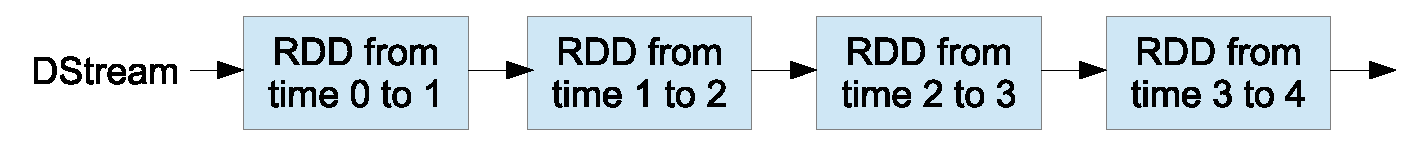
\includegraphics [width=1.0\textwidth]{images/SimpleDStream}
  \caption{Representation of a simple DStream.}
  \label{fig:SimpleDStream}
\end{figure}

Every operation you want to apply to DStream is applyed to every RDD object in the stream.
This implies, that transformation on the DStream produces new DStream.
All these transformation are executed by Spark Engine in a standard batch fashion.
Figure~\ref{fig:DStreamWithTransformation} depicts how it works.

\begin{figure}[H]
  \centering
  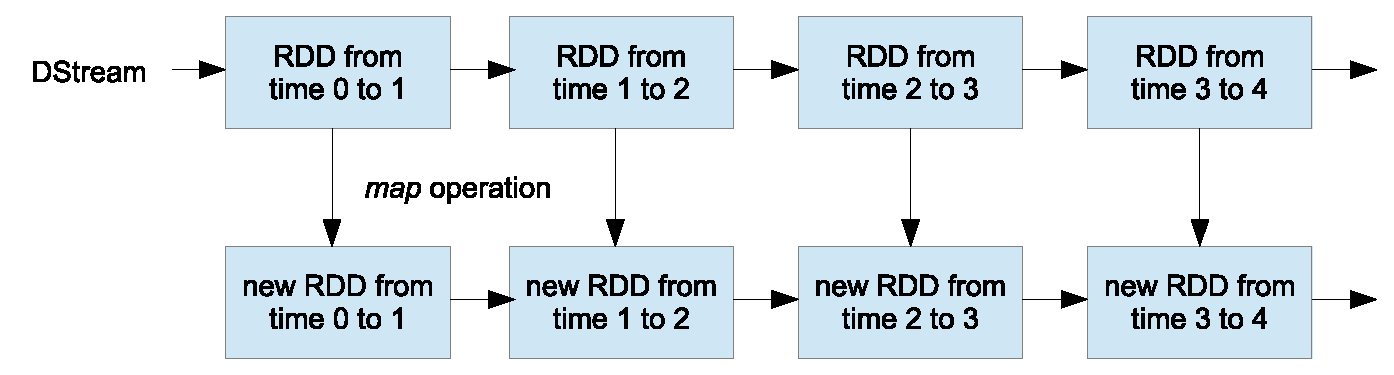
\includegraphics [width=1.0\textwidth]{images/DStreamWithTransformation}
  \caption{Transformation of a DStream to a new DStream.}
  \label{fig:DStreamWithTransformation}
\end{figure}

\textit{Input DStream} is a stream of raw data coming to Spark from the outer source.
Sources can be of two types: basic sources and advanced sources.
Basic sources are sources, that available using standard streaming context API, e.g. files or sockets.
Advanced sources are available using specific libraries, for example Kafka message queue server.
There is a notion of $Receiver$, that is an object that receives data from the stream, put into Spark's memory, so that it is available for input DStream, associated with this Receiver.
Every DStream is responsible only for one input data stream.
You can create many DStreams for different input streams to receive data from different data sources in parallel.
Receiver is executing as a long running task, hence it occupies one core of the processor.
This implies, that there should be more cores then receivers in the system.

Transformations on DStreams (UpdateStateByKey Operation, Transform Operation, Window Operations) ???

Spark streaming has a number of output operations on DStreams, that used to push transformed data to outer systems.
This can be files or databases.
Output operations actually start execution, as $actions$ of Spark engine do.
Examples of output operations are $print$, $saveAsObjectFiles$, $saveAsTextFiles$, $saveAsHadoopFiles$, $foreachRDD$.

DStream allows to persist it in the memory, when multiple computations of the same DStream are required.
Method $persist$ of DStream object does that.
Its execution specifies that every RDD of the DStream will be persisted in the memory, as it is done for RDD in Spark engine.
For data, arriving from network, the persistence level is so, that all data is replicated to two nodes to provide fault-tolerance.

There is a mechanism of checkpointing in Spark streaming.
It allows to make snapshots of intermediate data to HDFS.
It makes computation throughput less, if set not properly.
So it must be carefully tuned.

Fault-tolerance of Spark streaming is based on the fault-tolerance on Spark engine.
RDDs are basic elements of a DStream, what lets Spark streaming to rely on their robustness.
As long as all data locates on HDFS, if data node fails, all lost data can be recovered.
For data coming from network input stream, as we already mentioned, it is always replicated to two nodes.